%%%%%%%%%%%%%%%%%%%%%%%%%%%%%%%%%%%%%%%%%
% Beamer Presentation
% LaTeX Template
% Version 1.0 (10/11/12)
%
% This template has been downloaded from:
% http://www.LaTeXTemplates.com
%
% License:
% CC BY-NC-SA 3.0 (http://creativecommons.org/licenses/by-nc-sa/3.0/)
%
%%%%%%%%%%%%%%%%%%%%%%%%%%%%%%%%%%%%%%%%%

%----------------------------------------------------------------------------------------
%	PACKAGES AND THEMES
%----------------------------------------------------------------------------------------

\documentclass[xcolor=svgnames]{beamer}

\mode<presentation> {

% The Beamer class comes with a number of default slide themes
% which change the colors and layouts of slides. Below this is a list
% of all the themes, uncomment each in turn to see what they look like.

% \usetheme{default}
% \usetheme{AnnArbor}
% \usetheme{Antibes}
%\usetheme{Bergen}
% \usetheme{Berkeley}
% \usetheme{Berlin}
\usetheme{Boadilla}
% \usetheme{CambridgeUS}
% \usetheme{Copenhagen}
% \usetheme{Darmstadt}
% \usetheme{Dresden}
% \usetheme{Frankfurt}
% \usetheme{Goettingen}
% \usetheme{Hannover}
% \usetheme{Ilmenau}
% \usetheme{JuanLesPins}
% \usetheme{Luebeck}
% \usetheme{Madrid}
% \usetheme{Malmoe}
% \usetheme{Marburg}
% \usetheme{Montpellier}
% \usetheme{PaloAlto}
% \usetheme{Pittsburgh}
% \usetheme{Rochester}
% \usetheme{Singapore}
% \usetheme{Szeged}
% \usetheme{Warsaw}

% As well as themes, the Beamer class has a number of color themes
% for any slide theme. Uncomment each of these in turn to see how it
% changes the colors of your current slide theme.

% \usecolortheme{albatross}
% \usecolortheme{beaver}
%\usecolortheme{beetle}
% \usecolortheme{crane}
%  \usecolortheme{dolphin}
% \usecolortheme{dove}
% \usecolortheme{fly}
% \usecolortheme{lily}
% \usecolortheme{orchid}
% \usecolortheme{rose}
% \usecolortheme{seagull}
% \usecolortheme{seahorse}
% \usecolortheme{whale}
% \usecolortheme{wolverine}

% \setbeamertemplate{footline} % To remove the footer line in all slides uncomment this line
%\setbeamertemplate{footline}[page number] % To replace the footer line in all slides with a simple slide count uncomment this line

% \setbeamertemplate{navigation symbols}{} % To remove the navigation symbols from the bottom of all slides uncomment this line
}

\usepackage{graphicx} % Allows including imagesg
\usepackage{booktabs} % Allows the use of \toprule, \midrule and \bottomrule in tables
\usepackage{tikz}
\usepackage{multicol}
\usepackage{amsmath,amsthm,amssymb}
\usepackage{mathtools}
\DeclarePairedDelimiter\ceil{\lceil}{\rceil}
\DeclarePairedDelimiter\floor{\lfloor}{\rfloor}

\addtobeamertemplate{frametitle}{}{%
\begin{tikzpicture}[remember picture,overlay]
\node[anchor=north east,yshift=2pt] at (current page.north east) {
\includegraphics[height=0.8cm]{iiit-new.png}};
\end{tikzpicture}}

\setbeamercolor{title in head/foot}{bg=OrangeRed, fg=White}
\setbeamercolor{author in head/foot}{bg=RoyalBlue, fg=White}
\setbeamercolor{date in head/foot}{bg=SlateGray, fg=Black}

%----------------------------------------------------------------------------------------
%	TITLE PAGE
%----------------------------------------------------------------------------------------

\title[Discrete Structures]{Discrete Structures} % The short title appears at the bottom of every slide, the full title is only on the title page
\author{IIIT Hyderabad} % Your name
\institute[] % Your institution as it will appear on the bottom of every slide, may be shorthand to save space
{
Monsoon 2020 \\ % Your institution for the title page
\medskip
\textit{Tutorial 2} % Your email address
}
\date{September 21, 2020} % Date, can be changed to a custom date

\begin{document}

\begin{frame}
\titlepage % Print the title page as the first slide
\end{frame}

\begin{frame}
\frametitle{Introduction} % Table of contents slide, comment this block out to remove it
\tableofcontents % Throughout your presentation, if you choose to use \section{} and \subsection{} commands, these will automatically be printed on this slide as an overview of your presentation
\end{frame}

%----------------------------------------------------------------------------------------
%	PRESENTATION SLIDES
%----------------------------------------------------------------------------------------


%------------------------------------------------
\section{Questions}
%------------------------------------------------

%------------------------------------------------
\subsection{Question 0}
%------------------------------------------------
\begin{frame}
\frametitle{Question 0}
If $|A|$ = $m$ and $|B|$ = $n$ and $A$ and $B$ are not mutually disjoint. Let
\begin{align*}
\mathcal{P}_i(S) = \mathcal{P}(\mathcal{P}(\mathcal{P}\ldots \mathcal{P}(S)))) \text{  \textit{i}}  \text{    times}
\end{align*}
Comment on the value of $|\mathcal{P}_4(A-B) -  \mathcal{P}_2(A-B)|$. \\
\textbf{\underline{Sol.}} 
\begin{multicols}{2}
\begin{center}
    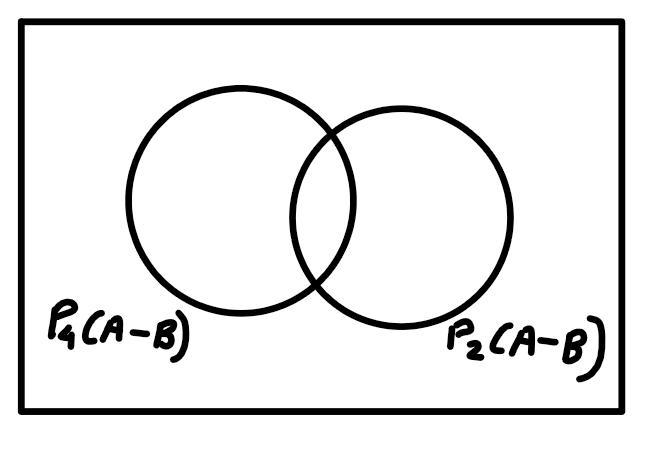
\includegraphics[width=0.9\linewidth]{photo_2020-09-22_22-35-08.jpg}
\end{center}

Let's denote $\mathcal{P}_2(A - B)$ as $C$. We get that, $P_4(A-  B)$  and $\mathcal{P}_2(A - B)$ will always the elements $\{\phi,\{\phi\}\}$. Thus the upper limit could be $2^{2^{2^{2^{m - 1}}}} - 2$. One of the lower limit could be $2^{2^{2^{2^{m - n}}}} - 2^{2^{m - n}}$
\end{multicols}
\end{frame}


%------------------------------------------------
\subsection{Question 1}
%------------------------------------------------
\begin{frame}
\frametitle{Question 1}
\textbf{1.1} Prove the following using basic set identities - 
\begin{enumerate}
    \item $((A - B) - (B - C))' = A' \cup B$ 
    \begin{align*}
        & ((A - B) - (B - C))' &  \\
        &= ((A \cap B') - (B \cap C'))' & \ldots \ldots \{\text{De Morgan's Law}\}\\
        &= ((A \cap B') \cap (B \cap C')')' & \ldots \ldots \{\text{De Morgan's Law}\} \\
        &= ((A \cap B') \cap (B' \cup C))' & \ldots \ldots \{\text{De Morgan's Law}\}\\
        &= ((A \cap B') \cap B') \cup ((A \cap B') \cup C))' & \ldots \ldots \{\text{Distributive Law}\} \\ 
        &= ((A \cap (B' \cap B')) \cup ((A \cap B') \cup C))' & \ldots \ldots \{\text{Associative Law}\}\\
        &= ((A \cap B') \cup ((A \cap B') \cup C))' & \ldots \ldots \{\text{Idempotent Law}\} \\
        &= ((A \cap B') \cap U) \cup ((A \cap B') \cup C))' & \ldots \ldots \{A \cap U = A\}\\
        &= ((A \cap B') \cap (U \cup C)))' & \ldots \ldots \{\text{Distributive Law}\}\\
        &= ((A \cap B'))' & \ldots \ldots A \cap U = A, A \cup U = A\} \\
        &= A' \cup B & \ldots \ldots \{\text{De Morgan's Law}\}\\
    \end{align*}
\end{enumerate}
\end{frame}
\begin{frame}
\begin{enumerate}\addtocounter{enumi}{1}
    \item $\big(A \cap (A - B )\big)\cup(A' \cup B)'= A - B$ 
    \begin{align*}
        & \big(A \cap (A - B )\big)\cup(A' \cup B)' &  \\
        &= \big(A \cap (A \cap B' )\big)\cup(A \cap B') & \ldots \ldots \{\text{De Morgan's Law}\}\\
        &= \big((A \cap A) \cap B' )\big)\cup(A \cap B') & \ldots \ldots \{\text{Associative Law}\} \\
        &= (A \cap B')\cup(A \cap B') & \ldots \ldots \{\text{Idempotent Law}\}\\
        &= (A \cap B') & \ldots \ldots \{\text{Idempotent Law}\} \\ 
        &= (A - B) & \ldots \ldots \{\text{De Morgan's Law}\}
    \end{align*}    
    \item $A \cup (B - C) = (A \cup B) - (C - A)$
    \begin{align*}
        &A \cup (B - C) \\
        &= A \cup (B \cap C') & \ldots \ldots \{\text{De Morgan's Law}\} \\
        &= (A \cup B) \cap (A \cup C') & \ldots \ldots \{\text{Distributive Law}\} \\
        &= (A \cup B) \cap (A' \cap C)' & \ldots \ldots \{\text{De Morgan's Law}\} \\ 
        &= (A \cup B) - (C - A) & \ldots \ldots \{\text{De Morgan's Law}\}
    \end{align*}
\end{enumerate}
\end{frame}
\begin{frame}
\begin{enumerate}\addtocounter{enumi}{3}
\item $(A \Delta B) \Delta C = A \Delta (B \Delta C) $ \\
\textbf{\underline{Sol:}} Part of Assigment 1, solutions will be posted after it.
\end{enumerate}
\end{frame}
\begin{frame}
\textbf{1.2} Prove the following using element of argument - 
\begin{enumerate}
    \item $(A \times B) \cap (C \times D) = (A \cap C) \times (B \cap D)$
    \begin{align*}
       &(x,y) \in (A \times B) \cap (C \times D) &\\
       &\implies  ((x,y) \in (A \times B)) \land ((x,y) \in (C \times D)) &\\
       &\implies  (x \in A \land y \in B) \land (x \in C \land y \in D) &\\
       &\implies  (x \in A \land x \in C) \land (y \in B \land y \in D) &\\
       &\implies  (x \in (A \cap C)) \land (y \in (B \cap D) &\\
       &\implies  (x,y) \in (A \cap C) \times (B \cap D)&
    \end{align*}
    Thus we have $(A \times B) \cap (C \times D) \subseteq (A \cap C) \times (B \cap D)$
    \begin{align*}
       &(x,y) \in (A \cap C) \times (B \cap D) &\\
       &\implies  (x \in A \land x \in C) \land (y \in B \land y \in D) &\\
       &\implies  (x \in A \land y \in B) \land (x \in C \land y \in D) &\\
       &\implies  (x,y) \in (A \times B) \land (x,y) \in (C \times D) &\\
       &\implies  (x,y) \in (A \times B) \cap (C \times D)&
    \end{align*}
    Thus we have $ (A \cap C) \times (B \cap D)  \subseteq (A \times B) \cap (C \times D)$
\end{enumerate}
\end{frame}
\begin{frame}
\begin{enumerate}\addtocounter{enumi}{1}
    \item $(A \times B) \cup (C \times D) \subseteq (A \cup C) \times (B \cup D)$  
    \begin{align*}
       &(x,y) \in (A \times B) \cup (C \times D) &\\
       &\implies  ((x,y) \in (A \times B)) \lor ((x,y) \in (C \times D)) &\\
       &\implies  (x \in A \land y \in B) \lor (x \in C \land y \in D) &\\
       &\implies  (x \in A \land x \in C) \land (y \in B \land y \in D) &\\
       &\implies  (x \in (A \cap C)) \land (y \in (B \cap D) &\\
       &\implies  (x,y) \in (A \cap C) \times (B \cap D)&
    \end{align*}
    Thus we have $(A \times B) \cup (C \times D) \subseteq (A \cup C) \times (B \cup D)$  
\end{enumerate}
\end{frame}


\subsection{Question 2}
\begin{frame}
\frametitle{Question 2}
\textbf{2.1}: Odd one out (ONLY ONE)
\begin{enumerate}
    \item $\{(a,b) | (a^2 = 1) \land (b^2 = 4)\}$
    \item $\{-1,-2,2,4\}$
    \item $(\{-1,1\} \times \{-2,2\}) - \phi$
    \item $(\{-1,1\} \times \{-2,2\}) \cup \phi$
\end{enumerate}
\textbf{\underline{Sol:}} \textbf{Option 2} \\
All others denote the set \{(-1,-2),(-1,2),(1,-2),(1,2)\}.
\end{frame}

%------------------------------------------------

\begin{frame}
\textbf{2.2}: Select the false statements:
\begin{enumerate}
    \item $\mathcal{P}(A \times B) = \mathcal{P}(A) \times \mathcal{P}(B)$
    \item $\mathcal{P}(A \cap B) = \mathcal{P}(A) \cap \mathcal{P}(B)$
    \item $\mathcal{P}(A \cup B) = \mathcal{P}(A) \cup \mathcal{P}(B)$
    \item $\mathcal{P}(A - B) = \mathcal{P}(A) - \mathcal{P}(B)$
\end{enumerate}
\textbf{\underline{Sol:}} \textbf{Option 1,3 and 4} \\ 
For options 1 and 3, take $A = \{a,b\}, B = {c}$. For option 3, take $A = \{a,b\}, B = \{b\}$ to disprove. It can be noted that in option 4, the element $\phi$ will get subtracted and will thus never be equal to LHS. For option 2 - 
\begin{multicols}{2}
We will show both sides.
\begin{align*}
    &X \in P(A \cap B) \\
    &(\forall x \in X) ( x \in A \land x \in B) \\
    &(\forall x \in X) ( x \in P(A) \land x \in P(B)) \\
    &X \in P(A) \cap P(B)
\end{align*}
\begin{align*}
    &X \in P(A) \cap P(B) \\
    &(X \in P(A)) \land (X \in P(B)) \\
    &(\forall x \in X) (( x \in P(A)) \land (x \in P(B)) \\
    &(\forall x \in X) ( x \in A \land x \in B) \\
    &(\forall x \in X) ( x \in (A \cap B)) \\
    &X \in P(A \cap B)
\end{align*}
\end{multicols}

\end{frame}
\begin{frame}
    \textbf{2.4}: $|U| = 20, |A| = 10, |B| = 5, |C| = 5, |A \cap B| = 2, |A \cap C| = 4, |B \cap C| = 1, |A \cap B \cap C| = 1$.
\begin{enumerate}
    \item $|A \cap B' \cap C| $ \\
    \textbf{\underline{Sol:}} $|A \cap C| - |A \cap B \cap C| = 3$
    \item $|((A - B) \times C)|$ \\
    \textbf{\underline{Sol:}} $|A - B| \cdot |C| = |A \cap B'| \cdot |C| = (|A| - |A \cap B|) \cdot |C| = 40$
    \item $|(A \Delta B) \cup (B \Delta C) |$ \\ 
    \textbf{\underline{Sol:}}     
\begin{multicols}{2}
\begin{center}
    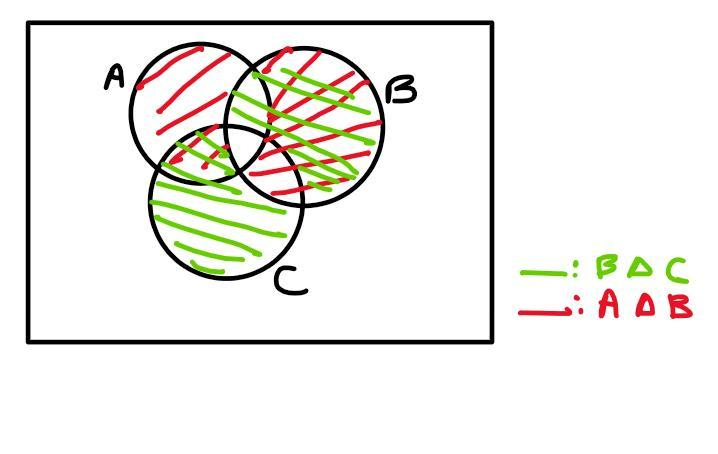
\includegraphics[width=\linewidth]{photo_2020-09-22_22-09-14.jpg}
\end{center}
From Venn Diagram it can be seen that it includes all regions within A, B and C except $A \cap B \cap C$. 
    Thus, it would be equal to $|A| + |B| + |C| - |A \cap B| - |A \cap C| - |B \cap C| = 13$
\end{multicols}    
    
\end{enumerate}

\end{frame}

%------------------------------------------------
\begin{frame}

\textbf{2.5}: Use inclusion exclusion principle to find numbers less than 1000 divisble by none of 2,3 or 5. 
\\ \textbf{\underline{Sol:}} We first find out the numbers divisible by 2,3 or 5.
\begin{align*}
    &\floor{\frac{999}{2}} + \floor{\frac{999}{5}} + \floor{\frac{999}{3}} - \floor{\frac{999}{10}} - \floor{\frac{999}{15}} - \floor{\frac{999}{6}} + \floor{\frac{999}{30}} \\
    &= 499 + 199 + 333 - 99 - 66 - 166 + 33 \\  
    &= 733
\end{align*}
So we would have rest as 999 - 733 = 266.
\end{frame}

\end{document} 